\documentclass[12pt,letterpaper,noanswers]{exam}
\usepackage[usenames,dvipsnames,svgnames,table]{xcolor}
\usepackage[margin=0.9in]{geometry}
\renewcommand{\familydefault}{\sfdefault}
\usepackage{multicol}
\pagestyle{head}
\header{AM 111 Class 10}{}{Interpolation, p.\thepage}
\runningheadrule
\headrule
\usepackage{siunitx}
\usepackage{graphicx} % more modern
\usepackage{amsmath} 
\usepackage{amssymb} 
\usepackage{hyperref}
\usepackage{tcolorbox}
\usepackage{enumitem}
\def\mbf{\mathbf}
\newcommand{\vc}[1]{\boldsymbol{#1}}
\def\dsst{\displaystyle}
\DeclareMathOperator*{\argmin}{arg\,min} % thin space, limits underneath in displays


\begin{document}
 \pdfpageheight 11in 
  \pdfpagewidth 8.5in

\noindent 

\section*{Preliminaries}

\begin{itemize}
\itemsep0pt
\item Problem set 04 is due on Friday at noon.
\item There will be a skill check in class during Class 09.  The problem info is below.
\item Find all OH on Canvas.
\item Quiz 01 is on Thursday Oct 12.  There is quiz info on canvas.
\end{itemize}



\noindent\textbf{Big picture}

Today: Algorithms for finding a curve that directly passes through data points.

\vspace{0.2cm}
\hrule
\vspace{0.2cm}

\noindent \textbf{Skill check practice}

List the Chebyshev interpolation nodes $x_1, ..., x_n$ on $[-1,1]$ for $n = 3$ ($n$ will be $\leq 5$).


\vspace{0.2cm}
\hrule
\vspace{0.2cm}

\noindent \textbf{Skill check solution}

The nodes are given by $\cos k\pi/(2n)$ for $k$ odd (and $0< k < 2n$).  For $n=3$ we have $\cos \pi/6$, $\cos 3\pi/6$, $\cos 5\pi/6$.



\vspace{0.2cm}
\hrule
\vspace{0.2cm}


\section*{Error when interpolating a polynomial}
From Sauer \S 3.2
\begin{tcolorbox}
\begin{enumerate}
    \item Start with a function $f(x)$ and use it to generate data points $(x_1, y_1), ..., (x_n, y_n)$.
    \item Create an interpolating polynomial $P_{n-1}(x)$.
\end{enumerate}
The \textbf{interpolation error} at $x$ is $f(x) - P_{n-1}(x)$.
\end{tcolorbox}

\begin{enumerate}
\item Given $n$ points, assume we have an interpolating polynomial $P_{n-1}(t)$.  Add one more point, $(x,f(x))$ to create $P_n(t)$.  Using Newton basis functions, we have $P_n(t) = P_{n-1}(t) + c_n(t-x_1)(t-x_2)...(t-x_n)$ where $P_n(x) = f(x)$.
\begin{parts}
\item Let $h(t) = f(t) - P_{n-1}(t) - c_n(t-x_1)(t-x_2)...(t-x_n)$.  To isolate $c_n$, take the $n$th derivative of your expression.
\item Argue that $h(t) = 0$ at $t = x, x_1, x_2, ..., x_n$. ($n+1$ points)

Rolle's theorem states the following: let $h$ be a continuously differentiable function on the interval $[a,b]$ and assume that $h(a) = h(b)$.  Then there exists a number $c\in (a,b)$ such that $h'(c) = 0$.

\item Using Rolle's theorem, at how many points can you guarantee $h'$ is zero?

\item Using it again, at how many points can you guarantee $h''$ is zero?

\item Argue that there must be one point $c$ for which $h^{(n)}(c) = 0$ (where $c$ is between the smallest and largest of $x, x_1, x_2, ..., x_n$).

\item Substitute $c$ into your expression from part (a) to find $c_n = \frac{1}{n!}f^{(n)}(c)$.
\end{parts}

\end{enumerate}
The point $(x,f(x))$ was arbitrary, so we have $f(x) = P_{n-1}(x) + \dfrac{f^{(n)}(c)}{n!}(x-x_1)(x-x_2)...(x-x_n)$.  This tells us that the interpolation error is $\dfrac{f^{(n)}(c)}{n!}(x-x_1)(x-x_2)...(x-x_n)$

\subsection*{Runge phenomenon}

For evenly spaced $x_i$ the interpolation error has a characteristic `wiggle' called Runge phenomenon.

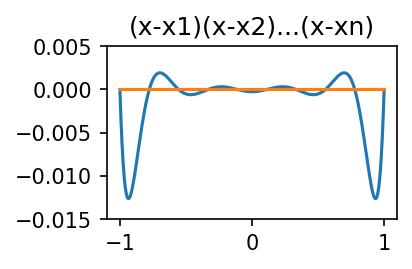
\includegraphics{AM111-F23-CourseNotes/img/C10-error.png}



\section*{Choosing the $x_k$ to minimize error}

When approximating a polynomial using interpolation, we can choose the $x_k$: they do not need to be selected to be evenly spaced.

Consider the interval $[-1,1]$ and the polynomial $(x-x_1)(x-x_2)...(x-x_n)$.

Theorem: the choice of real numbers $-1 \leq x_1,...,x_n\leq 1$ that makes the value of $\max\limits_{-1\leq x\leq 1}\left\vert (x-x_1)...(x-x_n)\right\vert$ as small as possible is $x_i = \cos\dfrac{(2i-1)\pi}{2n}$ for $i=1,...,n$ with a minimum value of $1/2^{n-1}$.

The minimum is achieved by $(x-x_1)...(x-x_n) = \dfrac{1}{2^{n-1}}T_n(x)$ where $T_n(x)$ denotes the degree $n$ Chebyshev polynomial.



\begin{enumerate}[resume]
\item The minimum is achieved by $(x-x_1)...(x-x_n) = \dfrac{1}{2^{n-1}}T_n(x)$ where $T_n(x)$ denotes the degree $n$ Chebyshev polynomial. 
Convince yourself that the $x_i$ are roots of $T_n(x)$.
\item How do the $x_i$ appear to be spaced in the Chebyshev case?

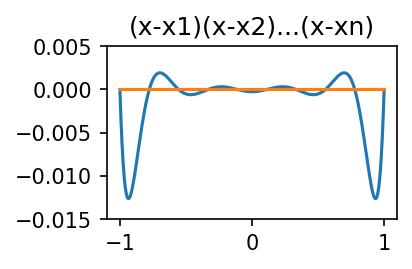
\includegraphics{AM111-F23-CourseNotes/img/C10-error.png}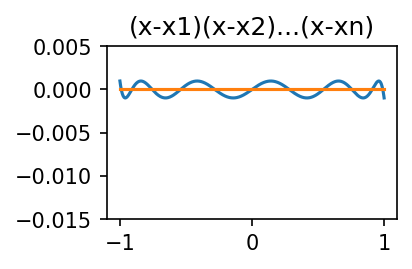
\includegraphics{AM111-F23-CourseNotes/img/C10-error-Ch.png}

\item Consider $f(x) = e^x$ on the interval $[-1,1]$.  Interpolate using $5$ points.

The interpolation error is $\dfrac{f^{(n)}(c)}{n!}(x-x_1)(x-x_2)...(x-x_5)$
\begin{parts}
    \item Find an upper bound for $f^{(5)}(x)$ on this interval.
    \item According to the Chebyshev theorem, $\vert (x-x_1)...(x-x_n)\vert \leq 1/2^{n-1}$.  Assuming five Chebyshev points, write a bound on the maximum value of $\vert (x-x_1)...(x-x_n)\vert$
    \item Write an expression for the maximum interpolation error if using Chebyshev roots for the $x_i$.
\end{parts}
\end{enumerate}
\subsection*{What are the Chebyshev roots?}
The $n$th Chebyshev polynomial is given by $T_n(x) = \cos(n\arccos x)$.

\begin{enumerate}[resume]
\item Find $T_0(x)$.
\item Find $T_1(x)$.
\item Let $y = \arccos x$ so that $\cos y = x$.  Write $T_2(x)$ in terms of $y$.

Use cosine identities to rewrite $T_2(x)$ in terms of $\cos y$ and find $T_2(x)$.
\end{enumerate}

$T_{n+1} = \cos((n+1)y) = \cos(ny + y)$.

$T_{n-1} = \cos((n-1)y) = \cos(ny - y)$.

We have $T_{n+1}(x) = \cos ny \cos y - \sin ny \sin y$ and $T_{n-1}(x) = \cos ny \cos y - \sin ny \sin (-y) = \cos ny \cos y + \sin ny \sin y$ so
$T_{n+1}(x) + T_{n-1}(x) = 2\cos(ny)\cos y$

\begin{enumerate}[resume]
\item $T_{n+1}(x) + T_{n-1}(x) = 2\cos(ny)\cos y$ where $\cos ny = T_n(x)$ and $\cos y = x$.  Write a recursion relation for $T_{n+1}(x)$ in terms of $T_n$ and $T_{n-1}$.
\end{enumerate}

Where are the roots of a Chebyshev polynomial?
\begin{enumerate}[resume]
\item Zeros are solutions of $0 = \cos(n\arccos x)$, so $n\arccos x = k\pi/2$ where $k$ is an odd integer.  
\begin{parts}
    \item Rearrange to find $x$.
    \item for $n = 4$ identify the roots.
\end{parts}
\end{enumerate}

Proof that the Chebyshev polynomial has the smallest maximum:  $T_n/2^{n-1}$ is monic (the coefficient of the highest order is $1$.  Let $P_n(x)$ be a monic polynomial with a smaller absolute maximum (so $\vert P_n(x)\vert < 1$ on $[-1,1]$).

There are $n+1$ points where $T_n$ is achieving $-1$ or $1$.  At these points, $P_n - T_n/2^{n-1}$ alternates between positive and negative.  That means there are at least $n$ zero crossings, and must have $n$ roots.  But $P_n - T_n/2^{n-1}$ is degree $\leq n-1$ so this is a contradiction.

\begin{enumerate}[resume]
\item Consider the following four interpolated polynomials fitting $e^{-(4x)^2}$.

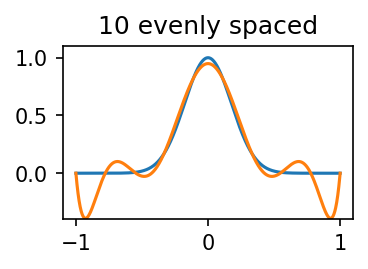
\includegraphics{AM111-F23-CourseNotes/img/C10-gaussian10.png}
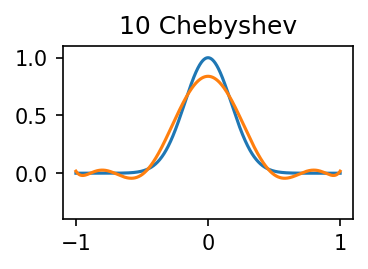
\includegraphics{AM111-F23-CourseNotes/img/C10-gaussian10Ch.png}

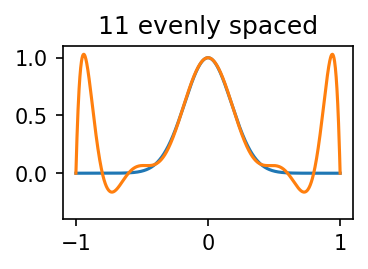
\includegraphics{AM111-F23-CourseNotes/img/C10-gaussian11.png}
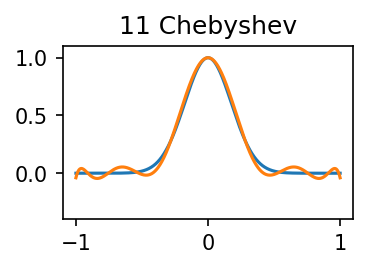
\includegraphics{AM111-F23-CourseNotes/img/C10-gaussian11Ch.png}

Match each to an error curve below:

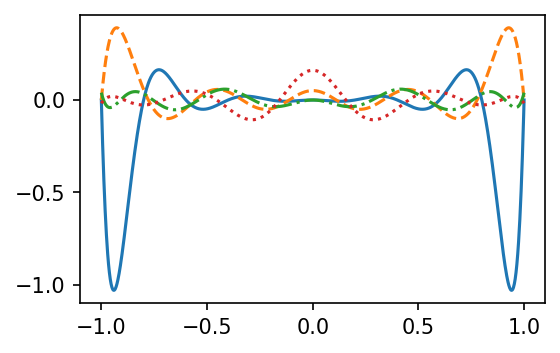
\includegraphics{AM111-F23-CourseNotes/img/C10-gaussianerror.png}

\end{enumerate}

\end{document}